\documentclass[12pt,a4paper]{article}

% ---------- Engine-safe font setup ----------
\usepackage{iftex}
\ifPDFTeX
  \usepackage[T1]{fontenc}
  \usepackage[utf8]{inputenc}
  \usepackage{tgheros}
  \renewcommand{\familydefault}{\sfdefault}
\else
  \usepackage{fontspec}
  \defaultfontfeatures{Ligatures=TeX,Scale=MatchLowercase}
  \IfFontExistsTF{Inter}{\setmainfont{Inter}}{\setmainfont{TeX Gyre Heros}}
\fi

% ---------- Layout & micro-typography ----------
\usepackage[margin=1.8cm]{geometry}
\usepackage{microtype}
\usepackage{ragged2e}
\usepackage{enumitem}
\setlist[itemize]{nosep,left=1.4em,topsep=1pt,itemsep=3pt}
\setlength{\parskip}{3.0pt}
\setlength{\parindent}{0pt}
\linespread{1.05}

% ---------- Colors (Spider-Man accents only) ----------
\usepackage{xcolor}
\definecolor{spiderRed}{HTML}{E11D2E}
\definecolor{spiderBlue}{HTML}{0E7AFE}
\definecolor{text}{HTML}{111827}
\definecolor{muted}{HTML}{667085}
\definecolor{rule}{HTML}{CBD5E1}

% ---------- Hyperref ----------
\usepackage{hyperref}
\hypersetup{
  colorlinks=true, urlcolor=spiderBlue, linkcolor=spiderBlue,
  pdfauthor={Pranay Kiran}, pdftitle={Pranay Kiran — Resume},
  pdfsubject={Professional Resume}, pdfkeywords={Resume, Engineering, Robotics, Automation, Mechanical, IoT},
  pdfcreator={JSON->LaTeX Resume Pipeline}, pdfproducer={latexmk/xelatex}
}
\urlstyle{same}

% ---------- Headings (bold black; super compact separator) ----------
\usepackage{titlesec}
\usepackage{tikz}
\usetikzlibrary{calc}
\newcommand{\SectionRule}{%
  \vspace{-6pt}
  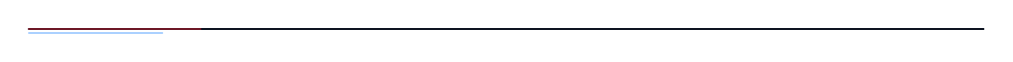
\begin{tikzpicture}[x=\linewidth,y=0.9pt]
    \draw[text!85!black, line width=0.8pt, line cap=round] (0,0) -- (1,0);
    \draw[spiderRed,  opacity=.45, line width=0.8pt, line cap=round] (0,0) -- (.18,0);
    \draw[spiderBlue, opacity=.35, line width=0.6pt, line cap=round] (0,-1.6) -- (.14,-1.6);
  \end{tikzpicture}%
  \vspace{-1pt}
}
\titleformat{\section}{\Large\bfseries\color{text}}{}{0pt}{}[\SectionRule]
\titlespacing*{\section}{0pt}{4pt}{0pt}

% ---------- FontAwesome optional (icons) ----------
\makeatletter
\IfFileExists{fontawesome5.sty}{\RequirePackage{fontawesome5}}{\newcommand{\faIcon}[1]{}}
\makeatother

% ---------- Skill chips ----------
\newcommand{\tagchip}[1]{%
  \tikz[baseline] \node[
    fill=spiderRed!8, text=spiderRed!95!black,
    rounded corners=2pt, inner xsep=4pt, inner ysep=1.6pt, anchor=base
  ]{\footnotesize #1};}

% ---------- Background (your positions/opacities) ----------
\usepackage{eso-pic}
\newcommand{\webOpacity}{0.18}
\newcommand{\iconsOpacity}{0.05}
\newcommand{\BackgroundIcons}{%
  \begin{tikzpicture}[remember picture,overlay]
    \node[text opacity=\iconsOpacity,anchor=center,text=spiderBlue!75!black]
      at ($(current page.center)+(-8.0,12.8)$) {\scalebox{7}{\faIcon{cogs}}};
    \node[text opacity=\iconsOpacity,anchor=center,text=spiderBlue!75!black]
      at ($(current page.center)+(-5.0,0.5)$) {\scalebox{6.5}{\faIcon{calculator}}};
    \node[text opacity=\iconsOpacity,anchor=center,text=spiderBlue!75!black]
      at ($(current page.center)+(6.0,6.8)$)  {\scalebox{6.5}{\faIcon{code}}};
    \node[text opacity=\iconsOpacity,anchor=center,text=spiderBlue!75!black]
      at ($(current page.center)+(6.0,-10.0)$) {\scalebox{7}{\faIcon{wrench}}};
  \end{tikzpicture}%
}
\newcommand{\webSize}{9.5cm}
\newcommand{\SpiderWebTR}{%
  \begin{tikzpicture}[remember picture,overlay]
    \begin{scope}
      \clip (current page.north west) rectangle (current page.south east);
      \begin{scope}[shift={($(current page.north east)+(-0.95cm,-0.95cm)$)}]
        \tikzset{webstrand/.style={spiderRed!60!black, line width=0.14pt, line cap=round, opacity=\webOpacity}}
        \tikzset{webring/.style={spiderRed!55!black, line width=0.16pt, line cap=round, opacity=\webOpacity}}
        \tikzset{webrim/.style={spiderRed!45!black, line width=0.18pt, line cap=round, opacity=\webOpacity}}
        \foreach \theta in {180,186,...,270}{ \draw[webstrand] (0,0) -- (\theta:\webSize+0.15cm); }
        \foreach \r in {0.70,1.15,1.60,2.05,2.50,2.95,3.40,3.90,4.40,4.95,5.55,6.20,6.90,7.60,8.35,9.15}{
          \draw[webring] (178.4:\r cm) arc[start angle=178.4, end angle=271.6, radius=\r cm];
        }
        \foreach \r in {1.4,3.1,5.1,7.3,9.0}{
          \draw[webrim] (180.8:\r cm) arc[start angle=180.8, end angle=269.2, radius=\r cm];
        }
      \end{scope}
    \end{scope}
  \end{tikzpicture}%
}
\AddToShipoutPictureBG*{\BackgroundIcons \SpiderWebTR}

% ---------- Footer build stamp ----------
\usepackage{fancyhdr}
\pagestyle{fancy}
\fancyhf{} \renewcommand{\headrulewidth}{0pt} \renewcommand{\footrulewidth}{0pt}
\fancyfoot[C]{\footnotesize\textit{\color{muted}Build: 2025-09-28 20:45 IST \,\,|\,\, hash: fc7cbba658}}
\setlength{\footskip}{13pt}

% ---------- Top underline ----------
\newcommand{\SplitUnderline}[2]{%
  \begin{tikzpicture}[baseline, x=\linewidth, y=1pt]
    \draw[line width=#2, color=text!90!black, line cap=round] (0,0) -- (1,0);
    \draw[line width=#2, color=spiderRed, opacity=.5, line cap=round] (0,0) -- (#1,0);
  \end{tikzpicture}%
}

% ---------- Header + education macros ----------
\newcommand{\NameFont}{\fontsize{23}{26}\selectfont\bfseries}
\newcommand{\ContactFont}{\normalsize}
\newcommand{\ExperienceEntry}[3]{%
  \noindent\begin{tabular*}{\linewidth}{@{}l@{\extracolsep{\fill}}r@{}}
    \textbf{#1} & {\small #3}\\[-2pt]
    \textit{#2} & \\
  \end{tabular*}\par
}
\newcommand{\EducationEntry}[3]{%
  \noindent\textbf{#1} --- #2%
  \if\relax\detokenize{#3}\relax\else\\\textcolor{muted}{#3}\fi
  \par\vspace{2pt}
}

\begin{document}
\color{text}
\justifying

% ---------- Header ----------
\noindent
\begin{minipage}{0.60\linewidth}
  {\NameFont Pranay Kiran}\\[-1pt]
  \small\textcolor{muted}{\textbf{Code + Mechanical = My Engineering Advantage}}
\end{minipage}%
\hfill
\begin{minipage}{0.38\linewidth}\raggedleft
  {\ContactFont \href{mailto:pranay@weberq.in}{pranay@weberq.in} \textcolor{muted}{\textbar} +91-1234567890 \textcolor{muted}{\textbar} \href{https://weberq.in}{weberq.in}}
\end{minipage}

\vspace{3pt}
\SplitUnderline{0.86}{1.1pt}

% ===================== Body (single column) =====================
\section*{Summary}
\small Multidisciplinary engineer with 5+ years of professional experience in aerospace, robotics, automation, and full-stack development. Proven expertise in establishing lithium battery production lines, automating manufacturing processes, and delivering product solutions from design to deployment.

\section*{Skills}
\textbf{Engineering:} Mechanical Design, Aerospace Analysis, Robotics \& Automation, Thermal Battery Design, Manufacturing Setup \\
\textbf{Software:} Python, Perl, PHP, Go, SQL/MySQL, Django, Flask, DevOps/Server Automation \\
\textbf{Electronics/IoT:} ESP32, Arduino, PCB Design, IoT Firmware \& Systems \\
\textbf{CAD:} NX, SolidWorks, Fusion 360, FreeCAD \\
\textbf{Analysis:} Structural (FEA), Fluid/Aero (CFD) \\
\textbf{Soft Skills:} Project Management, Cross-disciplinary Leadership, Quick Learner, Mentoring

\vspace{2pt}
\small \textcolor{muted}{\tagchip{Robotics}\ \tagchip{Thermal Batteries}\ \tagchip{Automation}\ \tagchip{IoT}\ \tagchip{DevOps}}

\section*{Programming Languages}
Python, Perl, PHP, Go, SQL/MySQL, Java (basic), JavaScript (basic), C/C++ (basic)

\section*{Experience}
\ExperienceEntry{Design Manager (Mechanical Design)}{Renewable Energy Systems Limited}{2023 – Present}
\begin{itemize}
\item Delivered full-scale lithium production capability
\item Increased throughput with IoT-guided automation
\item Improved reliability via glovebox and argon dryer designs
\item Led design of thermal batteries, jigs, and glovebox systems
\item Established lithium battery production line (civil, automation, gloveboxes)
\item Introduced IoT \& robotics for automated assembly
\end{itemize}


\ExperienceEntry{Technical Chairperson}{MLR CIE Incubation Center}{2022 – 2023}
\begin{itemize}
\item Mentored student startups and prototypes
\item Organized workshops and demos, improving innovation culture
\end{itemize}


\ExperienceEntry{Secretary}{Service to Mankind (NGO)}{2018 – 2021}
\begin{itemize}
\item Improved administration and event execution
\item Strengthened record management and stakeholder coordination
\end{itemize}


\section*{Projects}
\textbf{Assembly Guidance System \& Robotic Arm Automation} \\ IoT guidance LEDs for operators, scaled to a robotic arm with AI-assisted sequencing. \\ \textcolor{muted}{ESP32, Custom PCB, Firmware, Robotics}
\begin{itemize}
  \item Reduced training needs
  \item Eliminated errors
  \item Boosted throughput
\end{itemize}

\textbf{Lithium Plant Establishment} \\ End-to-end lithium line setup: gloveboxes, argon dryer towers, process automation.
\begin{itemize}
  \item Built in-house lithium capability
  \item Improved safety and reliability
\end{itemize}

\textbf{Full-Stack Banking Application} \\ Startup project: built and maintained full banking platform with DevOps automation.
\begin{itemize}
  \item Production-ready system
  \item Automated deployment
  \item Secure user flows
\end{itemize}

\textbf{Hydrogen Fuel Cell Prototype} \\ Academic project on automotive fuel cell stack design and integration.

\section*{Achievements}
\begin{itemize}
  \item Established lithium battery production line from scratch
  \item Automated assembly with IoT \& robotics
  \item Delivered production-ready banking application
  \item Contributed to Android ROMs \& NGO systems
\end{itemize}

\section*{Education}
\EducationEntry{Matriculation}{Genius High School}{9.3 / 10 (GPA)}
\EducationEntry{Intermediate}{Sri Chaitanya Junior College}{73\% (Percentage)}
\EducationEntry{B.Tech Mechanical Engineering}{MLR Institute of Technology}{7.8 (GPA)}
\EducationEntry{M.Tech Aerospace Engineering (in-progress)}{MLR Institute of Technology}{1 year completed}

\section*{Languages}
\textbf{Spoken:} Telugu, Hindi, English, French (basic)

\section*{Roles of Interest}
Mechanical Design Lead, Robotics \& Automation Engineer, Aerospace Structures Engineer

\end{document}
